%---------------------------------------------------------------------
%
%                          PeptideAtlas 1
%
%---------------------------------------------------------------------


\chapter*{\href{http://www.ncbi.nlm.nih.gov/pubmed/23811049}{A \textit{Candida albicans} PeptideAtlas}}
\addcontentsline{toc}{chapter}{A \textit{Candida albicans} PeptideAtlas}
%\cabeceraEspecial{A \textit{\textit{Candida albicans}} PeptideAtlas}
\addcontentsline{lof}{chapter}{A \textit{Candida albicans} PeptideAtlas}
\addcontentsline{lot}{chapter}{A \textit{Candida albicans} PeptideAtlas}


%\renewcommand{\headrulewidth}{0pt}
\cabeceraEspecial{A \textit{Candida albicans} PeptideAtlas}

\subsubsection*{Vital Vialas, Zhi Sun, Carla Ver\'onica Loureiro y Penha, Montserrat Carrascal, Joaqu\'in Abi\'an, Luc\'ia Monteoliva, Eric W. Deutsch, Ruedi Aebersold, Robert L. Moritz, Concha Gil}
\subsubsection*{Journal of Proteomics 2014, 97, 62-68}

%\subsubsection*{\href{http://www.ncbi.nlm.nih.gov/pubmed/23811049}{PMID: 23811049}}

\bigskip
\hfill
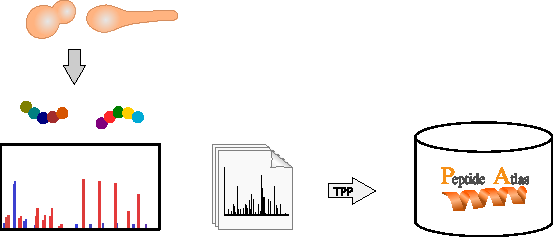
\includegraphics[width=1\textwidth]{Imagenes/Vectorial/graphical_abstract_PeptideAtlas1}



\newpage


%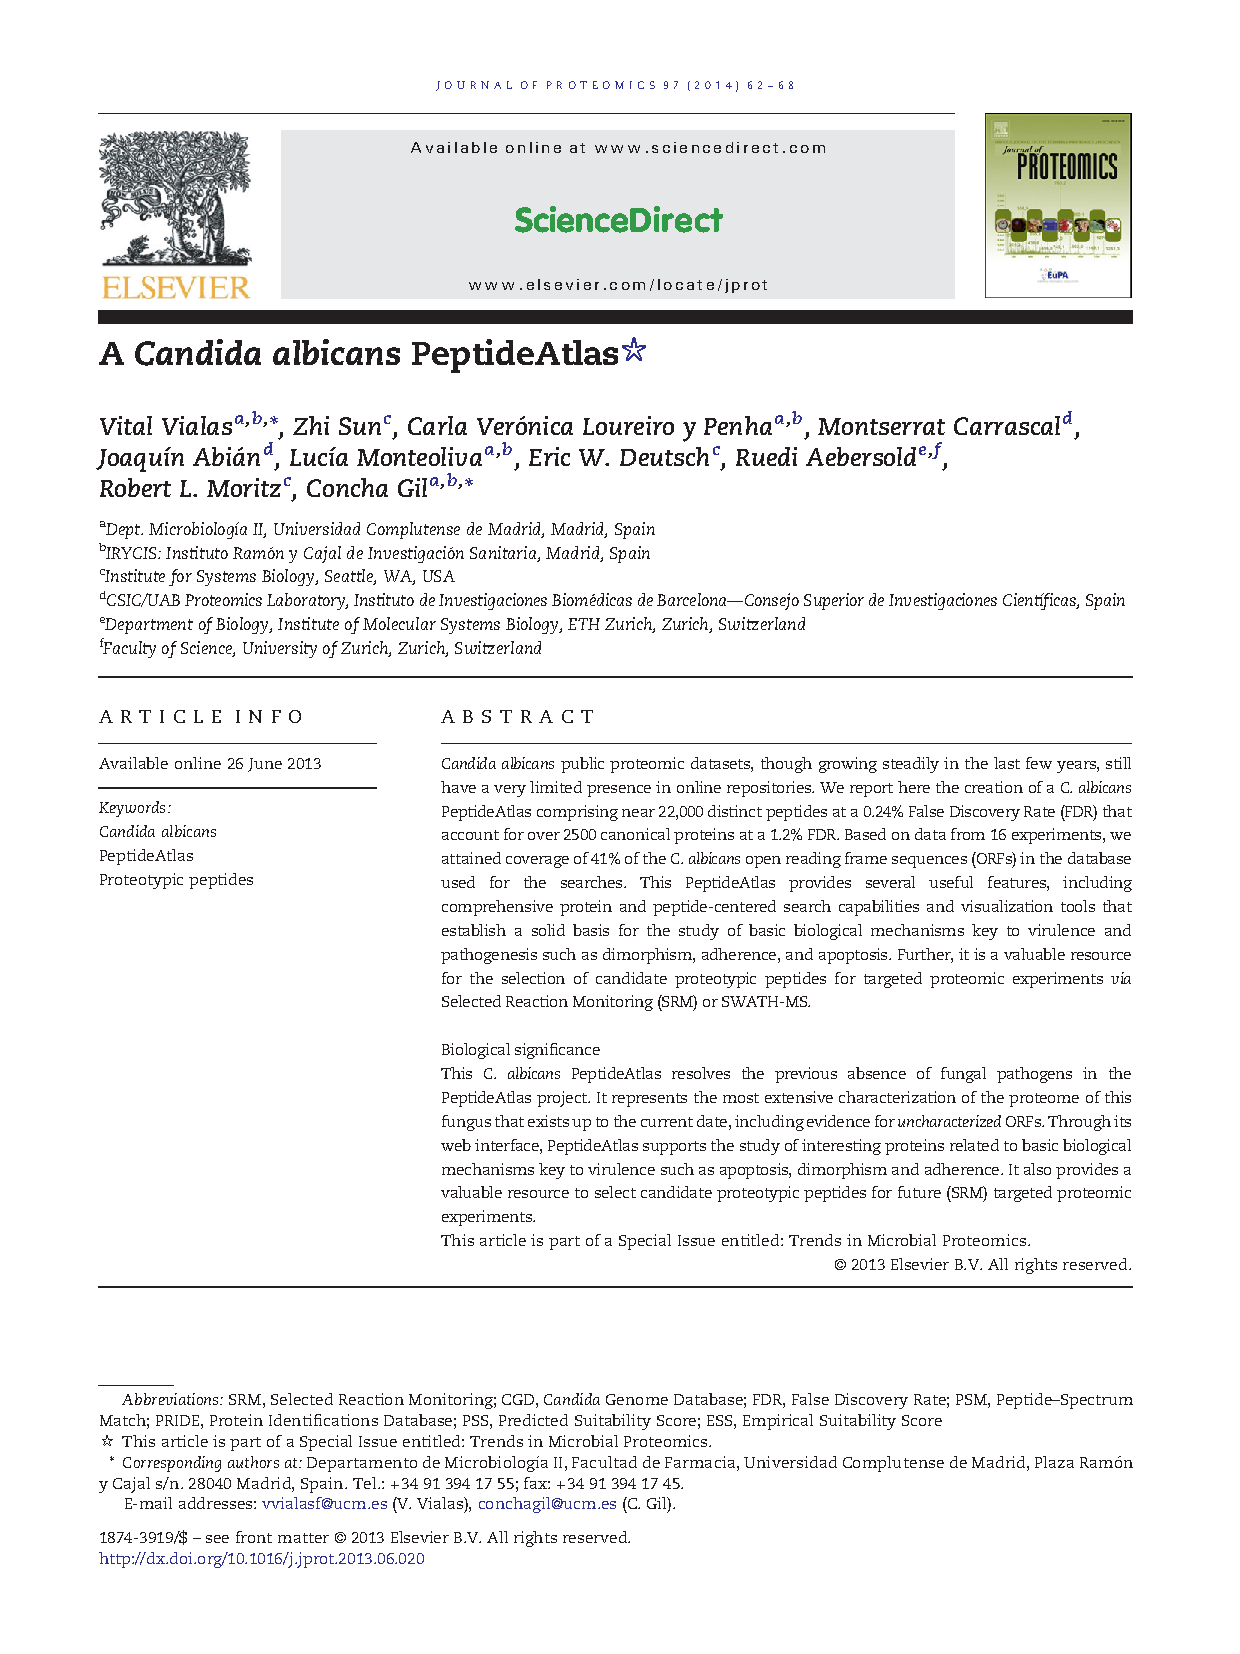
\includepdf[pages=-,scale=.8,pagecommand={}]{PeptideAtlas/Vialas_2013_PeptideAtlas_JProteomics.pdf}
%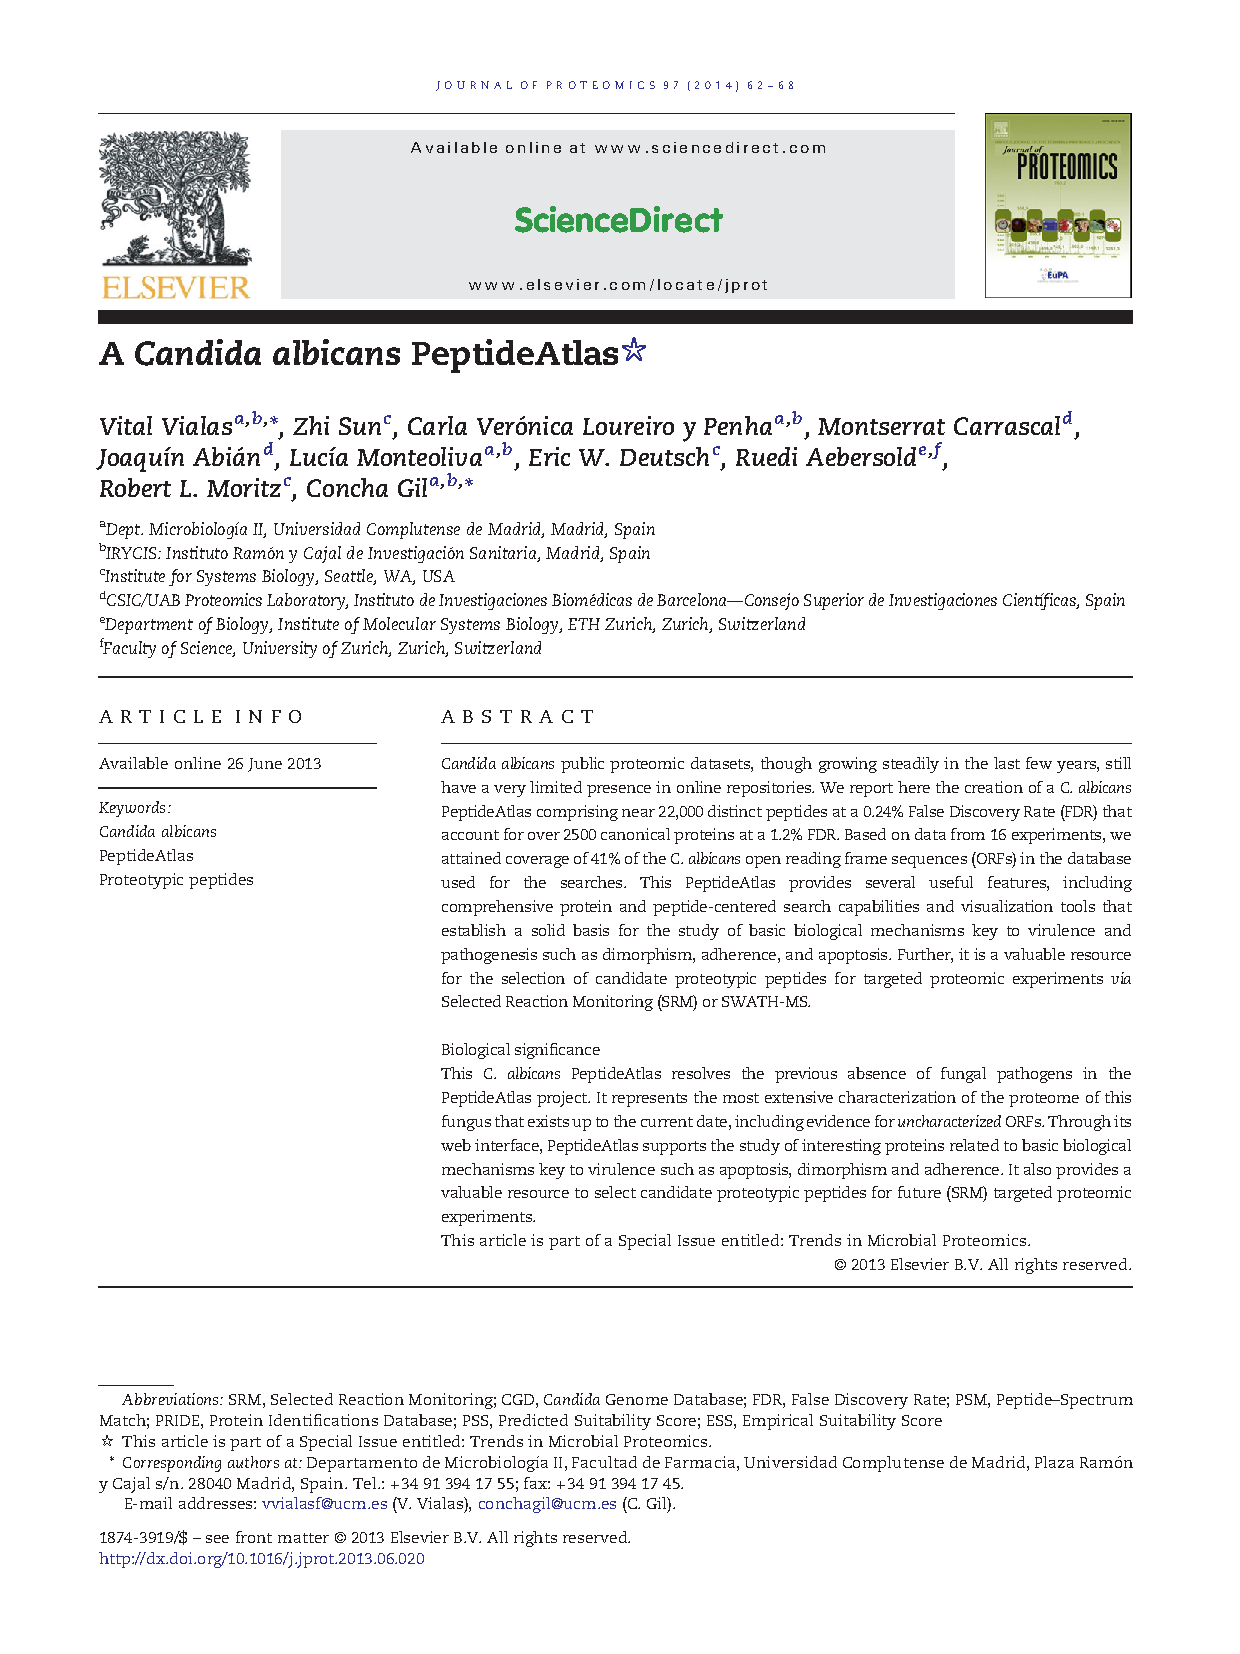
\includepdf[pages=-,pagecommand={}]{PeptideAtlas/Vialas_2013_PeptideAtlas_JProteomics.pdf}



\chapter*{Abstract}
\textit{Candida albicans} public proteomic datasets, though growing
 steadily in the last few years, still have a very limited presence in
 online repositories. We report here the creation of a \textit{\mbox{C. albicans}} PeptideAtlas
 comprising near 22,000 distinct peptides at a 0.24\% False Discovery
 Rate (FDR) that account for over 2500 canonical proteins at a 1.2\% FDR.
 Based on data from 16 experiments, we attained coverage of 41\% of the 
 \textit{\mbox{C. albicans}} open reading frame sequences (ORFs) in the database used 
 for the searches. This PeptideAtlas provides several useful features, 
 including comprehensive protein and peptide-centered search 
 capabilities and visualization tools that establish a solid basis for 
 the study of basic biological mechanisms key to virulence and 
 pathogenesis such as dimorphism, adherence, and apoptosis. 
 Further, it is a valuable resource for the selection of candidate 
 proteotypic peptides for targeted proteomic experiments via Selected
 Reaction Monitoring (SRM) or SWATH-MS

\subsection*{Biological Significance}
This \textit{\mbox{C. albicans}} PeptideAtlas resolves the previous absence of fungal 
pathogens in the PeptideAtlas project. It represents the most extensive
characterization of the proteome of this fungus that exists up to the 
current date, including evidence for uncharacterized ORFs. Through its 
web interface, \mbox{PeptideAtlas} supports the study of interesting proteins 
related to basic biological mechanisms key to virulence such as 
apoptosis, dimorphism and adherence. It also provides a valuable 
resource to select candidate proteotypic peptides for future (SRM) 
targeted proteomic experiments. 
This article is part of a Special Issue entitled: Trends in Microbial Proteomics.

\newpage


\phantomsection{}
\section*{Introduction}
\addcontentsline{toc}{section}{Introduction}

\textit{Candida albicans} is a fungus of great clinical importance. In
addition to asymptomatically colonizing mucous membranes
as a commensal in a large percentage of the population, it
may cause severe opportunistic infections in specific cases
such as patients with weakened immune defenses, a common
circumstance in cancer and AIDS patients. \textit{\mbox{C. albicans}} infections
are also a threat to patients in post-surgical situations and
intensive care unit stays. In this respect, invasive candidiasis
remains nowadays one of the major types of nosocomial
infections and a challenge in terms of economical and health
costs \citep{Wisplinghoff2004, Moran2010, Tong2008}.
From the perspective of proteomics, recent studies
have provided new insights into the \textit{\mbox{C. albicans}} biology and
suggested new clinical biomarker candidates for diagnosis and
prognosis of invasive candidiasis \citep{Pitarch2006, Pitarch2006a,
Fernandez-Arenas2007, Pitarch2011}.

However, the clinical relevance of this organism is not
reflected in the number of large-scale publicly available proteo-
mics resources. Up to the current date, the PRIDE \citep{Vizcaino2013} database
includes only 15 experiments accounting for 1786 identified
proteins. The more \textit{\mbox{C. albicans}}-focused Proteopathogen database
\citep{Vialas2009b} comprises several hundred protein identifications including
data from gel based proteomics, and other major proteomic
online resources such as the Global Proteome Machine Database 
(GPMDB \citep{Craig2004}) or Tranche \citep{Smith2011} contain no \textit{\mbox{C. albicans}} data
whatsoever.

As for the genomic data, according to \textit{Candida} Genome
Database (CGD), currently the most comprehensively annotated
\textit{\mbox{C. albicans}} sequence repository \citep{Costanzo2006a}, the \textit{\mbox{C. albicans}} genome
contains 6215 ORFs (as of May 28, 2013), out of which 1497 are
annotated as verified, i.e. representing genes for which there is
empirical evidence that the ORF actually encodes a functionally
characterized protein. In contrast, 4566 ORFs are termed
uncharacterized, indicating that there exists no conclusive evidence 
for the existence of a protein product. This data implies
that most part of the predicted proteome, over 70\% of the ORFs, is
still unknown or has not been properly annotated yet. An
extensive characterization of the \textit{\mbox{C. albicans}} proteome will
therefore be of great value to increase our knowledge in proteins
involved in mechanisms of virulence and infection and, thus
serves as a basis to design strategies for diagnosis, vaccination
and treatment of invasive candidiasis.

Since its inception, the PeptideAtlas project \citep{Desiere2006} has 
encouraged mass spectrometry data submission by the community and
has thus grown to a large compilation of atlases of different
species including human tissue and body fluid specific builds
(brain, plasma \citep{Farrah2011} and urine), microbial builds (\textit{Halobacterium} \citep{Van2008a},
\textit{Mycobacterium tuberculosis} \citep{Schubert2013}, \textit{Streptococcus} \citep{Lange2008},
\textit{Leptospira}, \textit{Plasmodium} \citep{Lindner2013}, \textit{Saccharomyces} \citep{King2006}
and \textit{Schizosaccharomyces} \citep{Gunaratne2013b});
invertebrate builds (\textit{Caenorhabditis elegans}, \textit{Drosophila} \citep{Loevenich2009} and
\textit{Apis mellifera} \citep{Chan2011}); and a pig and a bovine milk \citep{Bislev2012} builds. The
PeptideAtlas project, as a multi-species compendium of
proteomes, is continuously increasing its biological diversity.
The recent  \textit{Schizosaccharomyces pombe} atlas \citep{Gunaratne2013b} attains a large
coverage of its proteome by ad hoc extensive fractionation and
high-resolution LC-MS/MS, and contributes in the sense that
some of the fission yeast biological processes have a high degree
of conservation with the corresponding pathways in mammalian
cells. The incorporation of \textit{\mbox{C. albicans}} resolves the previous
absence of fungal pathogens in the PeptideAtlas and their under
representation in any public proteomic data repository.

Furthermore, the proven utility of PeptideAtlas as a resource
for selecting proteotypic peptides for Selected Reaction Monitoring (SRM)
 \citep{Deutsch2008} or SWATH-MS \citep{Gillet2012} will enable a starting point
for future targeted proteomics workflows in \textit{\mbox{C. albicans}}.



\phantomsection{}
\section*{Materials and methods}
\addcontentsline{toc}{section}{Materials and methods}

\subsection*{Empirical data compilation}

Large amounts of mass spectrometry data corresponding to
many and diverse measurements of the \textit{\mbox{C. albicans}} proteome
initially intended for different purposes were assembled in order
to build the PeptideAtlas. A range of proteomic methods,
protocols and different biological conditions were used to
generate the data as shown in Table 1. These include membrane
protein extractions \citep{Cabezon2009}, morphological yeast to hypha transition
experiments \citep{Monteoliva2010} and phosphoprotein enrichment treatments.
The combination of these diverse datasets resulted in an
unprecedented overall coverage of the \textit{\mbox{C. albicans}} proteome.
Protein samples were obtained as previously described in \citep{Monteoliva2010}.
Briefly, cells of the clinical isolate SC5314 were grown in YPD
medium for standard growth, whereas hyphal form growth was
induced using either Lee medium pH 6.7 or heat-inactivated
fetal bovine serum. Protein extracts were then obtained by
mechanical cell disruption using either glass beads in the MSK
cell homogenizer or the Fast-Prep cell breaker. Protein digests
were obtained by trypsinization and separated via HPLC. All
spectra acquisition runs were performed by LC-MS/MS in a data-
dependent manner in different instruments and setups. Table 1
provides an overview of the experiments along with the
instruments used for the mass spectrometry and the corresponding
 number of raw spectra data files that were acquired.
 


\begin{table}[t]
\caption*{Table 1. List of experiments collected to construct the \textit{\mbox{C. albicans}} PeptideAtlas.}
\renewcommand{\arraystretch}{1.5}
\footnotesize
\centering
\begin{tabular}{l p{4cm} p{2cm} c c }
\hline
\#Exp & Sample \newline{} (as named in the web interface) & Labeling/treatment & Instrument type & \#raw files\\
\hline
1 & Calb\_acidic\_subproteome & - & LTQ & 3\\
2 & Calb\_memb & - & LTQ & 8\\
3 & SILAC\_phos\_OrbitrapVelos\_1 & SILAC. IMAC+TiO2 & OrbitrapVelos & 3\\
4 & SILAC\_phos\_OrbitrapVelos\_2 & SILAC. IMAC+TiO2 & OrbitrapVelos & 3\\
5 & SILAC\_phos\_OrbitrapVelos\_3 & SILAC. IMAC+TiO2 & OrbitrapVelos & 3\\
6 & SILAC\_phos\_OrbitrapVelos\_4 & SILAC. IMAC+TiO2 & OrbitrapVelos & 3\\
7 & SILAC\_phos\_OrbitrapXL\_1A & SILAC. IMAC & OrbitrapXL & 11\\
8 & SILAC\_phos\_OrbitrapXL\_1A\_TiO2 & SILAC. IMAC+TiO2 & OrbitrapXL & 5\\
9 & SILAC\_phos\_OrbitrapXL\_1B & SILAC. IMAC & OrbitrapXL & 6\\
10 & SILAC\_phos\_OrbitrapXL\_1B\_TiO2 & SILAC. IMAC+TiO2 & OrbitrapXL & 6\\
11 & SILAC\_phos\_OrbitrapXL\_2 & SILAC. IMAC & OrbitrapXL & 6\\
12 & SILAC\_phos\_OrbitrapXL\_3 & SILAC. IMAC & OrbitrapXL & 6\\
13 & SILAC\_phos\_OrbitrapXL\_4 & SILAC. IMAC & OrbitrapXL & 5\\
14 & Calb\_extract\_3TOF & - & Triple TOF & 2\\
15 & Hyphal\_extract\_OrbitrapVelos & - & Orbitrap Velos & 4\\
16 & Yeast\_extract\_OrbitrapVelos & - & Orbitrap Velos & 4\\
\end{tabular}
\end{table}
\addcontentsline{lot}{table}{Table 1}


 

In addition, raw MS data from unpublished, SILAC labeled
and phosphoprotein enriched samples generated from studies
focused on \textit{Candida} interaction with host immune cells and from
experiments studying the hyphal and yeast-form proteomes,
were added to the collection.



\subsection*{Peptide and protein identification}

PeptideAtlas ensures consistency and quality of the stored data
by processing the raw spectra sets by the Trans-Proteomic
Pipeline (TPP) \citep{Deutsch2010c}, a suite of software tools for processing
shotgun proteomic datasets. The TPP tools are run in a well-
established sequential pipeline spanning steps from creating
 appropriate standard files to be used as input by the
search engine to statistical validation of protein inference
and calculation of the False Discovery Rate (FDR).

The collected raw spectra files in different proprietary file
formats were converted to the standard format for mass
spectrometry output data mzML \citep{Martens2011}, searched using X!Tandem
\citep{Craig2004} with the K-score algorithm plug-in \citep{MacLean2006} and the output search
results were converted to the search engine-independent
pepXML format \citep{Keller2005}.

The target fasta sequence file used for the search was
obtained from the \textit{Candida} Genome Database (CGD) \citep{Costanzo2006a} (Assembly 21)

Common contaminants from the common Repository of
Adventitious Proteins (cRAP) were appended. Then for each of
these sequences, counterpart reversed decoy sequences were
appended.

PeptideProphet \citep{Keller2002} was then run on the search results to
model the distributions of correctly and incorrectly assigned
Peptide-to-Spectrum Matches (PSMs). It then assigns probabilities
of being correct for each PSM, yielding a sensitive and flexible
approach to report results in a comparable manner. Next,
iProphet \citep{Shteynberg2011} was used to combine additional sources of evidence
including multiple identifications of the same peptide across
spectra, experiments, and charge and modification states,
allowing a more precise integration of evidence supporting the
identification of each unique peptide sequence. ProteinProphet
\citep{Nesvizhskii2003} was then run to refine iProphet probabilities by adding the
information at the protein level, like the number of sibling
peptides within a protein and to compute final protein level
probabilities. The prophet tools together combine multiple layers
of evidence and refine the model iteratively to achieve an optimal
analysis of the data. Finally MAYU \citep{Reiter2009} estimated FDR at different
levels for each contributing experiment and for the entire dataset
based on the PSMs to decoy proteins.

This process followed the pipeline first implemented in the
construction of the human plasma PeptideAtlas described in
\citep{Farrah2011} and successfully applied to other builds such as the
bovine milk and mammary gland PeptideAtlas \citep{Bislev2012}.


\subsection*{Construction of the PeptideAtlas}

The PeptideAtlas building process calculates the cumulative
number of identified peptide and proteins across the experiments,
 gathers information on protein to genome location
mappings and estimates the peptides' Empirical Suitability
Score and Predicted Suitability Score (ESS and PSS). The genomic
mappings, since \textit{\mbox{C. albicans}} is not present in the Ensembl database,
 which is the default PeptideAtlas uses to that purpose, were
extracted from the generic feature file 
C albicans SC5314 versionA21 s02m05r10 features.gff
obtained from CGD.

An overview of how the different experiments contribute,
in terms of the number of identified spectra and peptides, to
the atlas build is depicted in Fig. 1.

Besides, and due to the particularly rich number of identifications
 in experiments aimed at the detection of phosphorylated proteins
  (experiments \#3 to \#13), a similarly processed
version of the PeptideAtlas was created including in this case
PTMProphet results which provide, alongside each modified
residue, the probability that the post-translational modification
is truly detected at that site.




\phantomsection{}
\section*{Results and discussion}
\addcontentsline{toc}{section}{Results and discussion}

\subsection*{Assessment of proteome coverage and functional \newline enrichment analysis}

The assembled proteomic datasets (Table 1) were subject to
uniform data processing in order to build the \textit{\mbox{C. albicans}}
PeptideAtlas. 

\begin{figure}[t]
\begin{center}
 \includegraphics[width=0.80\textwidth]%
				 {Imagenes/Vectorial/PeptideAtlas1_Figure1}
\caption*{Figure 1. Histogram showing the cumulative number of distinct
peptides in the \textit{\mbox{C. albicans}} PeptideAtlas. Each bar represents a
different experiment that has contributed to the build. Bar
width is proportional to the number of high confidence PSMs.
Height of the blue section of the bar represents the number of
distinct peptides in each experiment and total height of the bar
(red plus blue sections) indicates the cumulative number of
peptides. The order of experiments is the same as in Table 1.}
\end{center}
\end{figure}
\addcontentsline{lof}{figure}{Figure 1}

The PSM assignment and protein inference
processes were conducted by means of the consistent and
robust pipeline TPP. The prophet tools integrate various levels
of information and report identification results in statistical
terms so that spectrum assignments, peptide to protein
mappings and protein groups are statistically validated, leading
to an overall improved sensitivity for a defined FDR level. As a
result the generated \textit{\mbox{C. albicans}} PeptideAtlas comprises 21,938
peptides identified at a 0.24\% FDR allocated to 2562 proteins at a
1.2\% FDR, that is, a coverage of 41.3\% of the 6209 \textit{\mbox{C. albicans}}
translated ORF sequences from the fasta database used for
searches. While the presented instance of the \textit{\mbox{C. albicans}}
PeptideAtlas has reached unprecedented coverage, it does
not represent a final representation of the respective proteome.
Like other PeptideAtlas instances for other species, the
\textit{\mbox{C. albicans}} atlas will be expanded upon submission and
processing of new MS data generated in ongoing projects.




To determine the biological functions encompassed by the
covered part of the proteome in this PeptideAtlas a Gene
Ontology (GO) annotation enrichment analysis was carried out
for the list of all detected \textit{\mbox{C. albicans}} canonical proteins, 
excluding decoy hits, using the biological process ontology and
Genecodis software \citep{Tabas-Madrid2012}. Predictably, it generated a diverse array
of clusters heterogeneously annotated, among which the
largest in number of proteins are associated with the GO
terms oxidation-reduction process, cellular response to drug, pathogenesis
 and hyphal growth respectively (Fig. 2). The enrichment in
some very generic GO terms such as oxidation-reduction process,
cellular response to drug and translation supports the hypothesis
that the diversity of experiments assembled to build the atlas
provides a representative, unbiased subset of the \textit{\mbox{C. albicans}}
proteome. In contrast, the more precise groups resulting from
the analysis related to pathogenesis, hyphal growth and fungal-type
cell wall organization are consistent with the large contribution to
the atlas by the experiment aimed at identifying proteins from
cells in hyphal form and by the profusion of these sort of
annotations in the source database.


\begin{figure}[t]
\begin{center}
 \includegraphics[width=0.90\textwidth]%
				 {Imagenes/Vectorial/PeptideAtlas1_Figure2}
\caption*{Figure 2. Gene Ontology annotation enrichment analysis for 
both the covered and undetected proteome subsets. All shown GO
annotations correspond to the biological process ontology and 
were found significant for a p-value cut-off below 0.01.}
\end{center}
\end{figure}
\addcontentsline{lof}{figure}{Figure 2}



As for the set of proteins present in the fasta database used
for the searches that are not covered in the PeptideAtlas, they
were subject to a similar analysis and were found to be enriched
in annotations related to the transmembrane transport GO term
(Fig. 2). These proteins are not easily observed by LC-MS/MS
techniques as previously reported \citep{Gunaratne2013b}. Also, we observed
enrichment in regulation of transcription, DNA-dependent in the
undetected part of the proteome. Given the short life span and
low abundance of many transcription factors it is plausible that
they were not detected in the collected datasets and their under
representation in proteomic data has also been reported in other
proteomic studies and in PeptideAtlas instances from other
species \citep{Gunaratne2013b,Ding2013,Simicevic2013}. 
The low number of protein groups significant-
ly associated with GO annotations in the undiscovered set is
understandably due to the fact that 2460 out of 3665 of the
undetected protein sequences, roughly two thirds, correspond to
unnamed ORFs, meaning, that little is known about their
biological function.



In addition to the groups of functionally characterized proteins,
 this PeptideAtlas offers solid empirical evidence for the
existence of 1564 proteins, showing a ProteinProphet probability
score greater than 0.9, corresponding to uncharacterized ORFs in
the CGD database (i.e., one-third of all 4566 uncharacterized ORFs).


\subsection*{Proteins of interest. Case of use}


From the clinical angle, the characterization of the \textit{\mbox{C. albicans}}
proteome is focused on particular subproteomes, including
cell surface constituents, and the set of proteins involved in
the yeast-to-hypha transition. The cell wall, as the outermost
cell structure represents the contact surface with host cells
and therefore gathers many antigens, virulence factors and
Pathogen Associated Molecular Patterns (PAMPs) \citep{Vialas2012}. Proteins
involved in hyphal growth are also relevant in pathogenesis,
in the sense that hyphae have been proven as key for
invasiveness whereas the switch back to yeast form plays a
role in dissemination \citep{Saville2003}.


Within these groups, a selected set of proteins of interest
present in the atlas, are the adhesins from the ALS family with
a role in invasiveness Als2p and Als3p; those required for cell
wall biogenesis and organization glycosidases Phr1p, Phr2p
and Utr2p; mannosyltransferases Pmt1p, Pmt4 and Pmt6;
those involved in the cell-wall glucan metabolism Mp65p and
Ecm33p, and the hyphal cell wall constituents Hwp1, Csp37p
and Rbt1p.

Other relevant proteins in the atlas are the ones related to
apoptosis, since those would make an ideal target for the
treatment of invasive candidiasis. Among those, the atlas
contains Mca1p, Bcy1p, Ras1p and three unnamed ORFs with
orthologous in other species showing roles in the apoptotic
process (orf19.713, orf19.967 and orf19.7365).

For any particular proteins of interest, the PeptideAtlas
web interface provides tools to explore the data. A user can
browse through a set of protein and peptide-centric views as
illustrated in Fig. 3 for the specific case of Bgl2p, a cell wall
glucosyltransferase. Its corresponding observed peptides are
highlighted in the protein sequence and sorted by the
Empirical Suitability Score (ESS), which represents the proportion
 of the number of samples in which the peptide is
observed with regard to the number of samples in which the
original protein is observed. This parameter, in combination
with others, such as a number of protein mappings, genome
location and amino acid composition will help the user to
select candidate proteotypic peptides for a targeted proteomics
 (SRM, Selected Reaction Monitoring) experiment.


Concerning those cases where a selected protein of
interest is not observed in the selected build, the PeptideAtlas
also provides the Predicted Suitability Score (PSS), a value
resulting from the combination of different observability
prediction algorithms based upon physico-chemical properties
 derived from the amino acid composition and previous
training datasets as described in \citep{Mallick2007}.

The build that assembles the phosphoprotein enrichment
experiments may be of great potential interest to study biological
processes such as signal transduction, since it encompasses a
number of kinases and phosphatases. A total of 421 different
phosphopeptides were detected and allocated to 210 phosphoproteins.

The largest number of phosphorylation sites occurs in S,
410 phosphopeptides contain, at least, one phosphorylation in S;
79 phosphopeptides contain, at least, one phosphorylation in T;
and 10 phosphopeptides contain one phosphorylation in Y.

 \begin{figure}[H]
\begin{center}
 \includegraphics[width=0.95\textwidth]%
				 {Imagenes/Vectorial/PeptideAtlas1_Figure3}
\caption*{Figure 3. Protein- and peptide-centric views for Bgl2p are
depicted. Distinct observed peptides are ranked by the BestProb
parameter (representing the PeptideProphet probability). 
Of those, most probably, some will also be present in the following
Predicted Highly Observable Peptides table were peptides are ranked 
by PSS, a combination of different prediction algorithms. For
all observed peptides, spectra from the different experiments are also available.}
\end{center}
\end{figure}
\addcontentsline{lof}{figure}{Figure 3} 





\phantomsection{}
\section*{Conclusions}
\addcontentsline{toc}{section}{Conclusions}

This \textit{\mbox{C. albicans}} PeptideAtlas build provides empirical identification
 evidence for 21,938 unique peptides including 421
phosphopeptides at a 0.24\% peptide-level FDR that account for a
high-confidence set (as defined in \citep{Farrah2011}) of 2562 canonical proteins
at a 1.2\% protein-level FDR representing thus a significant
advance in the proteomic characterization of \textit{\mbox{C. albicans}}.
Through the web interface, an important set of tools are
made available to the scientific community, enabling a solid
foundation to study different basic biological processes like
dimorphism, signal transduction, apoptosis and the interaction
with the human host. Furthermore, its value as a resource for
proteotypic peptide selection is of great potential interest for
future SRM experiments.
The current version of the PeptideAtlas can be found
at: 
\href{https://db.systemsbiology.net/sbeams/cgi/PeptideAtlas/buildDetails?atlas_build_id=323}{https://db.systemsbiology.net/sbeams/cgi/PeptideAtlas/buildDetails?atlas\_build\_id=323}
and the version including PTM results at:\newline{}
\href{https://db.systemsbiology.net/sbeams/cgi/PeptideAtlas/buildDetails?atlas_build_id=324}{https://db.systemsbiology.net/sbeams/cgi/PeptideAtlas/buildDetails?atlas\_build\_id=324}


\section*{Acknowlegements}
The Proteomics Unit UCM-Parque Cient\'ifico de Madrid is a
member of the ProteoRed-Spanish National Institute for
Proteomics.
We are thankful to Mar\'ia Luisa Hern\'aez and Jose Antonio
Reales for helping in sample obtention from the hyphal and
yeast form protein extracts and to Antonio Serna for providing
the tandem mass spectra from the triple-TOF instrument. Also
Aida Pitarch helped in the preparation of the manuscript.
This work was supported by BIO 2009-07654 and BIO
2012-31767 from the Ministerio de Econom\'ia y Competitividad,
PROMPT (S2010/BMD-2414) from the Comunidad de Madrid, and
Instituto de Salud Carlos III, Subdirecci\'on General de Redes y
Centros de Investigaci\'on Cooperativa, Ministerio de Econom\'ia y
Competitividad, Spanish Network for Research in Infectious
Diseases (REIPI RD12/0015) -co-financed by the European
Development Regional Fund`\"A way to achieve Europe\" ERDF.
EWD, ZS, and RLM are supported in part by the National
Institute of General Medical Sciences, under Grant No. R01
GM087221, 2P50 GM076547/Center for Systems Biology, the
National Science Foundation MRI [Grant No. 0923536], the EU
FP7 grant 'ProteomeXchange' [Grant No. 260558], and by the
Luxembourg Centre for Systems Biomedicine and the University
of Luxembourg.
RA is supported in part by ERC advanced grant 'Proteomics
v3.0' (Grant No. 233226) of the European Union.


\phantomsection{}
\section*{References}
\addcontentsline{toc}{section}{References}


\begin{itemize}[leftmargin=*]

\item[]{
Bislev, S., Deutsch, E., and Sun, Z. (2012), A Bovine PeptideAtlas of milk and mammary gland
proteomes, Molecular \& Cellular Proteomics, 12(18), 2895-2899.
}

\item[]{
Cabez\'on, V., Llama-Palacios, A., Nombela, C., Monteoliva, L., and Gil, C. (2009), Analysis of
\textit{Candida albicans} plasma membrane proteome., Proteomics, 9(20), 4770-86.
}

\item[]{
Chan, Q. W. T., Parker, R., Sun, Z., Deutsch, E. W., and Foster, L. J. (2011), A honey bee
(\textit{Apis mellifera} L.) PeptideAtlas crossing castes and tissues., BMC genomics, 12(1), 290.
}

\item[]{
Costanzo, M. C., Arnaud, M. B., Skrzypek, M. S., Binkley, G., Lane, C., Miyasato, S. R., and
Sherlock, G. (2006), The \textit{Candida} Genome Database: facilitating research on 
\textit{Candida albicans} molecular biology., FEMS yeast research, 6(5), 671-84.
}

\item[]{
Craig, R. and Beavis, R. C. (2004), TANDEM: matching proteins with tandem mass spectra.,
Bioinformatics, 20(9), 1466-7.
}

\item[]{
Desiere, F., Deutsch, E. W., King, N. L., Nesvizhskii, A. I., Mallick, P., Eng, J., Chen, S., Eddes,
J., Loevenich, S. N., and Aebersold, R. (2006), The PeptideAtlas project., Nucleic acids
research, 34(Database issue), D655-8.
}

\item[]{
Deutsch, E., Lam, H., and Aebersold, R. (2008), Data analysis and bioinformatics tools for
tandem mass spectrometry in proteomics, Physiological genomics, 33(1), 18-25.
}

\item[]{
Deutsch, E. E. W., Mendoza, L., Shteynberg, D., Farrah, T., Lam, H., Tasman, N., Sun, Z.,
Nilsson, E., Pratt, B., Prazen, B., Eng, J. K., Martin, D. B., Nesvizhskii, A. I., and Aebersold,
R. (2010), A guided tour of the TransProteomic Pipeline, Proteomics, 10(6), 1150-1159.
}

\item[]{
Ding, C., Chan, D. W., Liu, W., Liu, M., Li, D., Song, L., Li, C., Jin, J., Malovannaya, A., Jung,
S. Y., Zhen, B., Wang, Y., and Qin, J. (2013), Proteome-wide profiling of activated 
transcription factors with a concatenated tandem array of transcription factor response elements,
Proceedings of the National Academy of Sciences of the United States of America, 110(17),
6771-6.
}

\item[]{
Farrah, T., Deutsch, E. W., Omenn, G. S., Campbell, D. S., Sun, Z., Bletz, J. a., Mallick, P., Katz,
J. E., Malmstrom, J., Ossola, R., Watts, J. D., Lin, B., Zhang, H., Moritz, R. L., 
and Aebersold, R. (2011), A high-confidence human plasma proteome reference set with estimated
concentrations in PeptideAtlas., Molecular \& Cellular Proteomics, 10(9), M110.006353.
}

\item[]{
Fern\'andez-Arenas, E., Cabez\'on, V., Bermejo, C., Arroyo, J., Nombela, C., Diez-Orejas, R.,
and Gil, C. (2007), Integrated proteomics and genomics strategies bring new insight into
\textit{Candida albicans} response upon macrophage interaction., 
Molecular \& cellular proteomics: MCP, 6(3), 460-478.
}

\item[]{
Gillet, L. C., Navarro, P., Tate, S., Rost, H., Selevsek, N., Reiter, L., Bonner, R., and Aebersold,
R. (2012), Targeted data extraction of the MS/MS spectra generated by data-independent
acquisition: a new concept for consistent and accurate proteome analysis., Molecular \&
Cellular Proteomics, 11(6), O111.016717.
}

\item[]{
Gunaratne, J., Schmidt, A., Quandt, A., Neo, S. P., Sarac, O. S., Gracia, T., Loguercio, S.,
Ahrne, E., Xia, R. L. H., Tan, K. H., Lossner, C., Bahler, J., Beyer, A., Blackstock, W., y
Aebersold, R. (2013), Extensive Mass Spectrometry-based Analysis of the Fission Yeast
Proteome: The \textit{Schizosaccharomyces pombe} PeptideAtlas, Molecular \& Cellular Proteo-
mics, 12 (6), 1741-1751.
}

\item[]{
Keller, A., Nesvizhskii, A. I., Kolker, E., and Aebersold, R. (2002), Empirical statistical model
to estimate the accuracy of peptide identifications made by MS/MS and database search.,
Analytical chemistry, 74(20), 5383-92.
}

\item[]{
Keller, A., Eng, J., Zhang, N., Li, X.-j., and Aebersold, R. (2005), A uniform proteomics MS/MS
analysis platform utilizing open XML file formats, Molecular systems biology, 1(August
2005), 2005.0017.
}

\item[]{
King, N. L., Deutsch, E. W., Ranish, J. A., Nesvizhskii, A. I., Eddes, J. S., Mallick, P., Eng, J.,
Desiere, F., Flory, M., Martin, D. B., Kim, B., Lee, H., Raught, B., and Aebersold, R. (2006),
Analysis of the \textit{Saccharomyces cerevisiae} proteome with PeptideAtlas., Genome biology,
7(11), R106
}

\item[]{
Lindner, S. E., Swearingen, K. E., Harupa, A., Vaughan, A. M., Sinnis, P., Moritz, R. L., and
Kappe, S. H. I. (2013), Total and putative surface proteomics of malaria parasite salivary
gland sporozoites., Molecular \& Cellular Proteomics, 12(5), 1127-43.
}

\item[]{
Loevenich, S. N., Brunner, E., King, N. L., Deutsch, E. W., Stein, S. E., Aebersold, R., and
Hafen, E. (2009), The \textit{Drosophila melanogaster} PeptideAtlas facilitates the use of peptide
data for improved fly proteomics and genome annotation., BMC bioinformatics, 10, 59.
}

\item[]{
MacLean, B., Eng, J., Beavis, R., and McIntosh, M. (2006), General framework for developing
and evaluating database scoring algorithms using the TANDEM search engine, 
Bioinformatics, 22(22), 2830-2832.
}

\item[]{
Mallick, P., Schirle, M., Chen, S. S., Flory, M. R., Lee, H., Martin, D., Ranish, J., Raught, B.,
Schmitt, R., Werner, T., Kuster, B., and Aebersold, R. (2007), Computational prediction of
proteotypic peptides for quantitative proteomics., Nature biotechnology, 25(1), 125-31.
}

\item[]{
Martens, L., Chambers, M., Sturm, M., Kessner, D., Levander, F., Shofstahl, J., Tang, W. H.,
Rompp, A., Neumann, S., Pizarro, A. D., Montecchi-Palazzi, L., Tasman, N., Coleman, M.,
Reisinger, F., Souda, P., Hermjakob, H., Binz, P.-A., and Deutsch, E. W. (2011), mzML-a
community standard for mass spectrometry data., Molecular \& cellular proteomics : MCP,
10(1), R110.000133.
}

\item[]{
Monteoliva, L., Martinez-Lopez, R., Pitarch, A., Hernaez, M. L., Serna, A., Nombela, C., Albar,
J. P., and Gil, C. (2011), Quantitative proteome and acidic subproteome profiling of \textit{Candida
albicans} yeast-to-hypha transition, Journal of Proteome Research, 10(2), 502-517.
}

\item[]{
Moran, C., Grussemeyer, C. A., Spalding, J. R., Benjamin, D. K., and Reed, S. D. (2010),
Comparison of costs, length of stay, and mortality associated with \textit{Candida glabrata} and
\textit{Candida albicans} bloodstream infections., American journal of infection control, 38(1), 78-
80.
}

\item[]{
Nesvizhskii, A. I., Keller, A., Kolker, E., and Aebersold, R. (2003), A statistical model for 
identifying proteins by tandem mass spectrometry., Analytical chemistry, 75(17), 4646-58.
}

\item[]{
Pitarch, A., Nombela, C., and Gil, C. (2006a), \textit{Candida albicans} biology and pathogenicity:
insights from proteomics., Methods of biochemical analysis, 49, 285-330.
}

\item[]{
Reiter, L., Rinner, O., Picotti, P., Huttenhain, R., Beck, M., Brusniak, M.-Y., Hengartner, M. O.,
and Aebersold, R. (2011), mProphet: automated data processing and statistical validation
for large-scale SRM experiments., Nature methods, 8(5), 430-5.
}

\item[]{
Saville, S. P., Lazzell, A. L., Monteagudo, C., and Lopez-Ribot, J. L. (2003), Engineered control
of cell morphology in vivo reveals distinct roles for yeast and filamentous forms of \textit{Candida
albicans} during infection., Eukaryotic cell, 2(5), 1053-60.
}

\item[]{
Schubert, O. T., Mouritsen, J., Ludwig, C., Rost, H. L., Rosenberger, G., Arthur, P. K., Claassen,
M., Campbell, D. S., Sun, Z., Farrah, T., Gengenbacher, M., Maiolica, A., Kaufmann, S. H. E.,
Moritz, R. L., and Aebersold, R. (2013), The Mtb Proteome Library: A Resource of Assays
to Quantify the Complete Proteome of \textit{Mycobacterium tuberculosis}., Cell host \& microbe,
13(5), 602-12.
}

\item[]{
Shteynberg, D., Deutsch, E. W., Lam, H., Eng, J. K., Sun, Z., Tasman, N., Mendoza, L., Moritz,
R. L., Aebersold, R., and Nesvizhskii, a. I. (2011), iProphet: Multi-level Integrative Analysis
of Shotgun Proteomic Data Improves Peptide and Protein Identification Rates and Error
Estimates, Molecular \& Cellular Proteomics, 10(12), M111.007690-M111.007690.
}

\item[]{
Simicevic, J., Schmid, A. W., Gilardoni, P. A., Zoller, B., Raghav, S. K., Krier, I., Gubelmann,
C., Lisacek, F., Naef, F., Moniatte, M., and Deplancke, B. (2013), Absolute quantification
of transcription factors during cellular differentiation using multiplexed targeted proteomics.,
Nature methods, advance on.
}

\item[]{
Smith, B. E., Hill, J. A., Gjukich, M. A., and Andrews, P. C. (2011), Tranche 
distributed repository and ProteomeCommons.org., Methods in molecular biology (Clifton, N.J.), 696,
123-45.
}

\item[]{
Tabas-Madrid, D., Nogales-Cadenas, R., and Pascual-Montano, A. (2012), GeneCodis3: a
non-redundant and modular enrichment analysis tool for functional genomics., Nucleic acids
research, 40(Web Server issue), W478-83.
}

\item[]{
Tong, K. B., Murtagh, K. N., Lau, C., and Seifeldin, R. (2008), The impact of esophageal 
candidiasis on hospital charges and costs across patient subgroups., Current medical research
and opinion, 24(1), 167-74.
}

\item[]{
Van, P. T., Schmid, A. K., King, N. L., Kaur, A., Pan, M., Whitehead, K., Koide, T., Facciotti,
M. T., Goo, Y. A., Deutsch, E. W., Reiss, D. J., Mallick, P., and Baliga, N. S. (2008), 
Halobacterium salinarum NRC-1 PeptideAtlas: toward strategies for targeted proteomics and
improved proteome coverage., Journal of proteome research, 7(9), 3755-64.
}

\item[]{
Vial\'as, V., Nogales-Cadenas, R., Nombela, C., Pascual-Montano, A., and Gil, C. (2009), 
Proteopathogen, a protein database for studying \textit{Candida albicans}-host interaction., 
Proteomics, 9(20), 4664-8.
}

\item[]{
Vial\'as, V., Perumal, P., Gutierrez, D., Xim\'enez-Emb\'un, P., Nombela, C., Gil, C., and Chaffin,
W. L. (2012), Cell surface shaving of \textit{Candida albicans} biofilms, hyphae and yeast form
cells., Proteomics, 12(14), 2331-2339.
}

\item[]{
Vizca\'ino, J. A., Cot\'e, R. G., Csordas, A., Dianes, J. a., Fabregat, A., Foster, J. M., Griss, J.,
Alpi, E., Birim, M., Contell, J., O Kelly, G., Schoenegger, A., Ovelleiro, D., P\'erez-Riverol,
Y., Reisinger, F., R\'ios, D., Wang, R., and Hermjakob, H. (2013), The PRoteomics IDEnti-
fications (PRIDE) database and associated tools: status in 2013., Nucleic acids research,
41(Database issue), D1063-9.
}

\item[]{
Wisplinghoff, H., Bischoff, T., Tallent, S. M., Seifert, H., Wenzel, R. P., and Edmond, M. B.
(2004), Nosocomial bloodstream infections in US hospitals: analysis of 24,179 cases from
a prospective nationwide surveillance study., Clinical infectious diseases : an official 
publication of the Infectious Diseases Society of America, 39(3), 309-17.
}



\end{itemize}
